
\section{Experiments}


% \begin{figure*}
%     \centering
%     \includegraphics[width=\linewidth]{figures/VA-benchmark.png}
%     \caption{\textbf{Variational Automation Benchmark Setup} that includes  Grocery Fulfillment (Simulation and Real), Grocery Packing (Simulation / Real), Popcorn Making (Simulation / Real), USB-C Cable Insertion (Real) and Industrial Crate Washing (Sim) }
%     \label{fig:benchmark-setup-fig}
% \end{figure*}

\subsection{Simulation and Real-World Variational Automation Benchmarks}
We present 8 VA benchmark tasks, including 4 in simulation and 4 in real-world.
Six of these are inspired by  LIBERO~\citep{liu2023libero}, the de facto standard for evaluating VLA policies in simulation.

\textbf{Benchmark (I-a,b): Fulfill Grocery Orders (Sim and Real)} Each instance of this task involves locating a designated target item and placing it into the basket. The original LIBERO~\cite{liu2023libero} benchmark did not vary the position of the  (\textit{objects}) which allows for overfitting to the demonstration examples. To address this, the {LIBERO-Pro}~\citep{zhou2025liberopro} evaluation suite swaps target and basket object positions at test time (\textit{object\_swap}). We introduce four extensions for our VA Benchmarks: 1) \textit{X-Y 20$\times$20 {\small{$cm^2$}}}, where the position of each object varies uniformly within a 20$\times$20 {\small{$cm^2$}} zone centered around the original LIBERO object pose; 2) \textit{basket\_swap}, which swaps the target item and basket location; 3) \textit{permutation}, which swaps target item and distractor item positions; and \textit{mixed\_all} including all three variation types. The physical benchmark directly mirrors this setup.
% , requiring the physical robot to successfully identify, grasp, and place the target object into the container. 
To avoid object collisions during task instance generation, we utilize Minkowski sum~\cite{minkowski1896geometrie} operations to ensure item singulation.  The real version of this benchmarks uses a Franka arm with wrist camera and  real items from a grocery store.  

\textbf{Benchmark (II-a,b): Pack Grocery Items (Sim and Real)} We modify Benchmark I-a,b to create multi-object pick-and-place tasks, as in a grocery checkout line, where the robot is assigned to pack 6 objects into a container without needing to identify or select any specific items. We quantify the success rate as the number of items (out of 6) placed into the basket after 6 grasping attempts. 

\textbf{Benchmark (III-a,b): Make Popcorn (Sim and Real)} We use the LIBERO frypan, stove, and knob assets to create a manipulation task that requires the robot to sequentially turn on a stove, pick up the pan handle, place it on the stove, remove the pan, and turn off the stove.  For the real version of this benchmark, we use the Franka Robot arm with wrist-camera, a portable stove from Amazon and Jiffy-Pop popcorn.

\textbf{Benchmark (IV): Insert Cables (Real)} This benchmark task requires a UR5 robot arm with with the ZED Mini wrist camera to execute a series of USB-C cable insertions and extractions in a bank of 6 sockets.  The robot uses internal force torque feedback to probe the insertion when the target port goes beyond the camera's field of view.  The benchmark includes two varying conditions. First, we vary the pose of the cable ports, testing three distances in 5 {\small{$cm$}} increments and three angles in 15° increments. Second, we vary the text prompt to specify five distinct goals: targeting individual ports, inserting in ascending order, descending order, odd-indexed ports, and even-indexed ports.  

% We conducted five trials for each configuration, yielding 130 
\textbf{Benchmark (V): Wash Crates (Sim) } This simulation benchmark simulates a real industrial crate-washing use case where two Franka robot arms must cooperatively grasp a crate by narrow slits on its sides, lift it off a stack, flip it, and place it onto a washing machine table.  Each instance varies the initial pose of the crate, varying yaw rotations of up to $\pm15^{\circ}$ and horizontal displacements of up to $\pm2.5$ {\small{$cm$}}.
The benchmark provides a language instruction \textit{``Cooperatively lift the top crate off the stack with both Franka arms, flip it over, and place it on the washing machine table,''}. (Fig.~\ref{fig:crate-wash-setup}).


%This benchmark simulates the automation of a real industrial crate washing use case with bi-manual robot picks, flips and places crate.  

\subsection{Baselines}
Each cell in Table 1 represents the outcome from trials with 100 task instances of Benchmarks I-a and II-a (in simulation) for a total of over 5000 simulation trials.  We run CaP-X~\cite{fu2026cap} which uses a single agent and is given only an image of the initial task instance and natural language instructions. We note that this is not a fair comparison as GaP is designed for Variational Automation where environment geometry is known (but object location is unknown), so the performance of CaP-X serves as an ablation of GaP with a single agent and without self-learning.  We evaluate VLA models $\pi_{0.5}$~\cite{black2025pi_} and MolmoAct2~\cite{fang2026molmoact2} with official checkpoints finetuned on the LIBERO training dataset. We also evaluate TipTop~\cite{shen2026tiptop}, a modular open-vocabulary planning system for robotic manipulation based on TAMP. We configure this from the github code with the default configuration of 128 particles for cuTAMP~\cite{shen2024differentiable} with a 60-second planning timeout.
We warm up the cuTAMP cache before measuring the execution time.  Rows 5 and 6 represent combinations of GaP with VLA models, where GaP generates an initial robot motion to center the wrist camera over the target object (bringing the VLA into distribution).

% We note that our GaP system utilizes additional inputs, specifically object geometry and scene configuration for internal simulation. Consequently, the performance of CaP-X effectively serves as an ablation of GaP, representing a single-agent approach devoid of our proposed graph structure.
For GaP and CaP-X, we use Gemini-3.1-Flash-Lite for LLM agents and VLM with a temperature of 0.1.  
For Benchmarks I and II,  GaP does not perform self-learning because the first graph generated achieves high performance.



\subsection{Benchmarks I and II: Fulfill Grocery Orders and Pack Grocery Items}


\begin{table}[t]
  \centering
  \footnotesize
  
  \caption{\scriptsize \textbf{Success Rates for 5500 trials, 100 task instances per table cell. Results on Benchmarks I-a and II-a: Fulfill Grocery Orders and Pack Grocery Items}. The first two columns are the original LIBERO~\cite{liu2023libero} with negligible pose variation, and LIBERO-PRO with slightly larger pose variation~\cite{zhou2025liberopro} . We introduce the VA Grocery Order Fulfillment benchmark that includes larger object positional variance (X-Y 20$\times$20 {\scriptsize{$cm^2$}}), swapping target and basket positions (basket\_swap), permuting all item locations, and everything combined (mixed\_all). We also introduce the Grocery Packing benchmark that requires picking all objects and placing them in the basket. In rows 5 and 6, GaP navigates the robot wrist camera above the target object and then switches to MolmoAct2 and $\pi_{0.5}$ VLA policies.  }
  \label{tab:benchmark-banked}
  \resizebox{\linewidth}{!}{%
  \begin{tabular}{lcccccccc}
  \toprule
   & LIBERO & LIBERO-Pro & \multicolumn{4}{c}{Fulfill Grocery Orders} & \multicolumn{2}{c}{Pack Grocery Items} \\
  \cmidrule(lr){2-2}\cmidrule(lr){3-3}\cmidrule(lr){4-7}\cmidrule(lr){8-9}
  Method & object & object\_swap & X-Y 20$\times$20 {\small{$cm^2$}} & basket\_swap & permutation & mixed\_all & fixed & varied \\
  \midrule
  CaP-X   & - & 0.22 & 0.07 & 0.05 & 0.11 & 0.10 & 0.01 & 0.01 \\
  $\pi_{0.5}$               & 0.96 & 0.24 & 0.78 & 0.15 & 0.20 & 0.20 &   0.17   &   0.18   \\
  MolmoAct2                 & \textbf{0.97} & 0.43 & 0.90  & 0.26 & 0.10 & 0.20 &  0.18    &    0.18 \\
  TipTop   & 0.22      &   0.22   &  0.29    &   0.24   &   0.31   &   0.24   &   0.34   &     0.46    \\
  \midrule
  $\pi_{0.5}$ w/GaP         & 0.85 & 0.60 & 0.79 & 0.32 & 0.50 & 0.39 &  0.67    &  0.66    \\
  MolmoAct2 w/GaP           & 0.70 & 0.62 & 0.84 & 0.58 & 0.39 & 0.66 &  0.59    &    0.59  \\
  GaP                       & {0.95} & \textbf{0.95} &  \textbf{0.95} & \textbf{0.97} & \textbf{0.93} & \textbf{0.97} &   \textbf{0.99 }  &  \textbf{0.98}    \\
  \bottomrule
  \end{tabular}%
  }
  \vspace{-10pt}
\end{table}
% \vspace{-5em}

% \eric{may need to change grocery packing to completion rate? the success rate is too low for baselines}
% \eric{describe how gap generate graph, skill used.}
\subsubsection{Simulation Results}
\textbf{GaP achieves significantly better positional robustness compared to baselines.} As shown in Table 1.   While baseline VLA models ($\pi_{0.5}$, MolmoAct2) achieve high success rates on LIBERO-object without pose variation, their performance drops as low as 0.20 for LIBERO-PRO with positional variance. In contrast, GaP maintains a robust success rates across all variations. We find that TipTop~\cite{shen2026tiptop} cannot generate motion plans for many of these benchmark task instances because M2T2~\cite{yuan2023m2t2}, cuRobo~\cite{sundaralingam2023curobo}, and cuTAMP~\cite{shen2024differentiable} cannot plan feasible solutions.

% \textbf{GaP shows robustness compared to alternative methods.} \eric{similarly for libero-packing}

\textbf{VLA policies can benefit from GaP.} Performance for $\pi_{0.5}$ w/GaP and MolmoAct2 w/GaP suggest that GaP can enhance robustness of existing VLA models as shown in rows 5 and 6 of Table 1. As VLA policies struggle with positional perturbation of target objects, GaP uses the wrist camera and interactive perception skills to reliably identify the target object and uses linear cartesian motion skills to navigate the arm and wrist camera to a pre-grasp pose above the target object. The GaP computation graph then hands over execution to the VLA policy.  GaP thus brings the VLA input into distribution, producing more than a twofold improvement in success rates. %for models like MolmoAct2 under highly randomized configurations. In some setups that are typically similar to training dataset (object and X-Y 20$\times$20 {\small{$cm^2$}}), the performance can drop because the hand-over pose may not be present in the training dataset.

\subsubsection{Real Physical Experiment Results}
\begin{wraptable}{r}{0.4\columnwidth}
  \centering
  \vspace{-\baselineskip}  % optional: tightens spacing above
  \scriptsize
  \caption{\scriptsize \textbf{Physical Benchmark on Benchmark I-b Fulfill Grocery Orders, Benchmark II-b Pack Grocery Items and Benchmark III-b Make Popcorn}. We report success rate and completion time. Sub-tasks ($\rightarrow$) are reported per benchmark. On average, the completion time of single pick-and-place for TipTop is 95 seconds, and GaP is 67 seconds. }
  % Completion Time & 95.0 s &  \textbf{67.0 s}\\
  
  \label{tab:benchmark-transposed}
  \resizebox{\linewidth}{!}{%
  \begin{tabular}{lrr}
  \toprule
  Success Rate & TipTop & GaP \\
  \midrule
  Fulfill Grocery Orders            & 8/25   & \textbf{25/25} \\
  \quad$\rightarrow$ object        & 3/5   & 5/5 \\
  \quad$\rightarrow$ 20x20         & 2/5   & 5/5 \\
  \quad$\rightarrow$ basket swap   & 1/5   & 5/5 \\
  \quad$\rightarrow$ tall basket   & 0/5  & 5/5 \\
  \quad$\rightarrow$ permutation   & 2/5   & 5/5 \\
  \midrule
  Pack Grocery Items                & 10 /30   & \textbf{28/30} \\
  \midrule
  Make Popcorn                &  0/ 20  & \textbf{18/20} \\
  \quad$\rightarrow$ pan pick and place   & 2/5  & 5/5 \\
  \bottomrule
  \end{tabular}%
  \label{tab:real}
  }
  \vspace{-8pt}
  \vspace{-\baselineskip} 
\end{wraptable}
\textbf{GaP transfers well from Sim to Real}. Table \ref{tab:real} 
% We use the identical graph generated in simulation and execute on a real-world setup. 
For the {Fulfill Grocery Orders} benchmark, GaP achieves a perfect success rate of 25/25 (100\%), while TipTop succeeds in only 8/25 trials. 
Both GaP and TipTop accurately identify the objects. However, TipTop~\cite{shen2026tiptop} fails because M2T2~\cite{yuan2023m2t2}, cuRobo~\cite{sundaralingam2023curobo}, and cuTAMP~\cite{shen2024differentiable} combined cannot find feasible motion plans for cubic-shaped objects, tall baskets, or varied object orientations.
% Furthermore, GaP proves to be more execution-efficient, reducing the average completion time by 29.5\%, from 95.0~s to 67.0~s. These results validate that the task graphs generated by GaP successfully transfer to physical hardware and exhibit robust generalization under real-world uncertainty.
In terms of execution time, GaP perceives the item and basket in parallel using 14.1 seconds to generate oriented bounding boxes, and 36.4 seconds for descending, grasping, and transporting the items.

\subsection{Ablation Studies}
For Fulfilling Grocery Orders and Packing Grocery Items, the full GaP system achieves robust success rates (0.93–0.99). We ablate as follows: (1) Graphless generation forces the LLM to perfectly inline low-level service interfaces, such as method names and request schemas, from memory. Consequently, even when the high-level logic is correct, minor syntax or interface mismatch errors inevitably terminate the trial.  So replacing the structured graph output with a single LLM that generates raw Python scripts collapses the success rate to zero.
(2) Condensing GaP's specialized authoring agents into a single LLM also drops success rates to zero, with all trials failing static structural verification prior to execution, because a single LLM agent struggles to simultaneously manage global data flow, local logic, and verification, frequently introducing dangling references or node collisions. Furthermore, even with iterative feedback, a single LLM tends to oscillate between mistake classes without converging. 
(3) {Graph validation improves graph connectivity}. For each configuration in Fulfill Grocery Orders, some task segmentation agents emit a first-attempt subgraph that fails static type/edge checks and would crash at runtime, for example, some graphs wire the input and output of the {transport} phase in drop-pose computation to the release phase and other is in checkpoint verification. GaP's graph validation verifies the wiring and effectively ensures the graph edge connectivity.


% Continual learning / iterative / mental rehearsal 
% graph edge selection and parameter tuning 
% compare with: 
% no graph validation at all
% + LLM as verifier + syntax checking (CAP-X (?))
% + graph validation (such as edge message validation)
% + simulation-based iterative learning 
% compare with conditions: providing perfect scenario (simulation directly), or real-to-sim (using RecGen + LLM Agent for simulation generation)


\subsection{Benchmark III a, b: Make Popcorn in sim and real}
% \eric{this part will be completed by Thursday - sorry but this will be our last minute experiment :( }
% \begin{figure}
%     \centering
%     
\includegraphics[width=0.8\linewidth]{figures/popcorn.png}
%     \caption{\textbf{Physical Setup (Left), Internal Graph Learning Simulation (Middle), and Convergence Data (Right) of long-horizon popcorn making } that requires the robot to turn the stove knob, pick up the pan handle, place and align the pan with the stove, and pick the pan after it is done.  \eric{placeholder figure, will replace with actual simulation setup and data}}
%     \label{fig:popcorn}
% \end{figure}

\begin{wrapfigure}{r}{0.5\columnwidth}
\centering
\vspace{-\baselineskip}
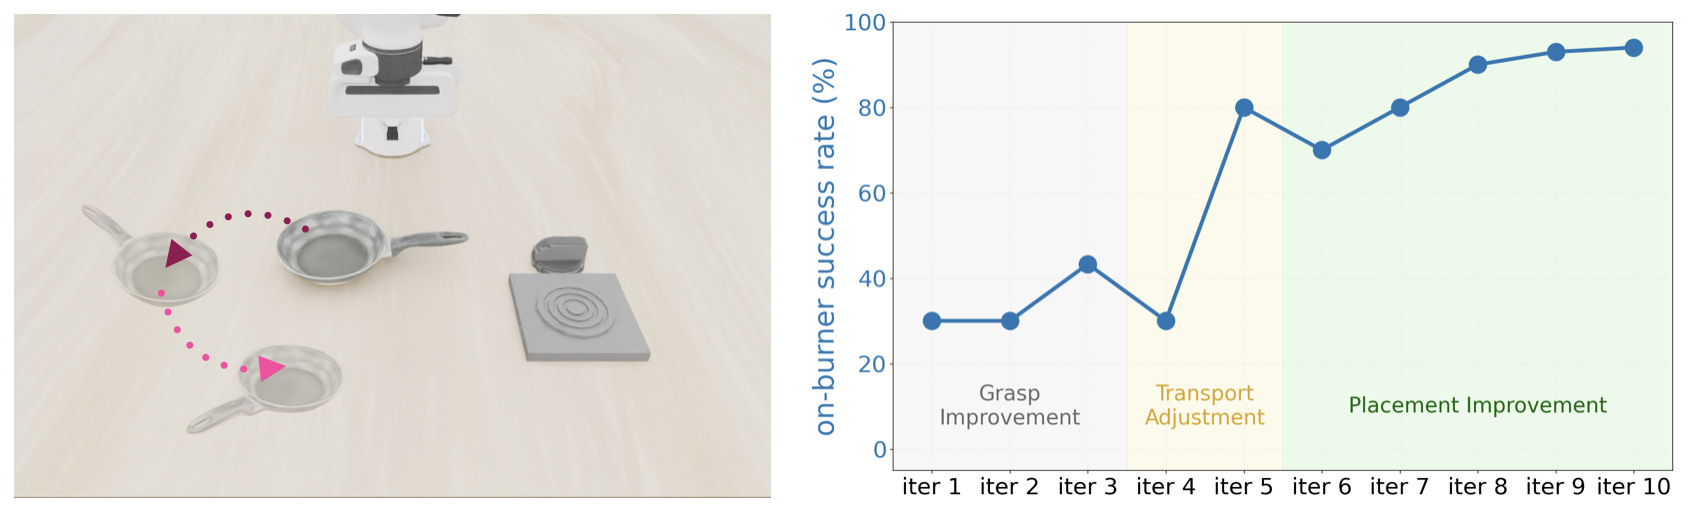
\includegraphics[width=\linewidth]{figures/rehearsal-new.png}
\caption{\scriptsize \textbf{Self-Learning for Making  Popcorn  Benchmark.}
Pan pose variations (left) drives an 10-iteration sequence graph update ; (blue, left axis) iteration phases shaded by class of edit.}
\label{fig:reh_res}
\vspace{-10pt}
\end{wrapfigure}
The Make Popcorn task requires the robot to grasps the stove knob and rotate it to turn on the burner, then the robot must find and pick up the handle of the JiffyPop popcorn pan, place it on the stove burner, wait, and then turn off the stove.

GaP generates a graph using GraspGen~\cite{murali2025graspgen}, knob turning skills and other object localization and grasping skills from Benchmark 1 and 2. 
The initial graph is able to turn on and off the knob but unable to pick and place the pan properly --  achieving only a 33\% success rate. 

\textbf{Self-Learning significantly increases success rate.} As shown in the Fig.~\ref{fig:reh_res}, self-learning proceeds through three stages: (1) from iteration 1 to 3, the majority of failures come from pan grasping failure, where the simulator feedback reports that the Franka gripper is not in contact with the object pan, so GaP replaces the GraspGen grasp skill with a skill that mixes GraspGen with an oriented bounding box grasp planner.
(2) In iteration 4, GaP  recognizes that the pan should be grasped by the handle, thereby adjusting the perception algorithm prompts to localize the pan handle.  
(3) In iterations 4-8, GaP finetunes the offset of pan placement due to the changed grasping strategy to align the pan with the stove surface. 

The resulting policy achieves 94\% in simulation with variations of pan position and orientation, and achieves a 90\% (18/20) success rate in real physical trials as shown in Table \ref{tab:real}. 
% The failure cases in simulation is caused by the kinematics infeasibility of top-down grasping pan handle strategy when the pan handle is away from the robot. The failure cases in real world is caused by an inverse kinematics error of linear cartesian motion, and another is a mis-grasp caused by   kinematics accumulation error of long-horizon rollout.
The two physical failures resulted from one inverse kinematics (IK) error during linear Cartesian motion, and one misgrasp caused by accumulated kinematic error.

% grasp moe, grasp gen, obb, select 
% iteration 1 -3  grasp gen -> obb -> grasp moe 
% transport method -> cartesian joint limit 
% change to short axis grasp to cartesian 
% and place with offset 

% , and use Newton simulator~\cite{Newton} 

 % \syx{ablation, running right now}

% \textbf{Simulation based iterative learning is more helpful than other vision based approach} One important observation is that simulation rollouts provide access to geometric states, including 3D world coordinates and object meshes, across scene variations. This helps prevent the generated graph from overfitting to a single visual configuration and enables more reliable diagnosis of failure causes. In contrast, a VLM-only approach~\syx{cite RoboSQ/Robo2VLM?} for node-level failure detection achieves only 71\% agreement with human judgments. Our simulation-based failure diagnosis achieves 98\% agreement with human judgments across 100 test cases. Accurate failure detection contributes to the successful graph update. \syx{ablation, running right now}

% \textbf{Multi-Agent System prevents agents from \textit{cheating}}

% \eric{ablation / baseline: compare with (1) using VLM instead of internal simulation state; (2) no simulation at all; (3) agent write checkpoint themselves (no multiagent) - cheating; (4) different LLM (?) }


\subsection{Benchmark IV: Insert Cables (Real)}

\begin{figure}[htbp]
    \centering
    
    % Left Side: The Figure
    \begin{minipage}{0.48\textwidth}
        \centering
        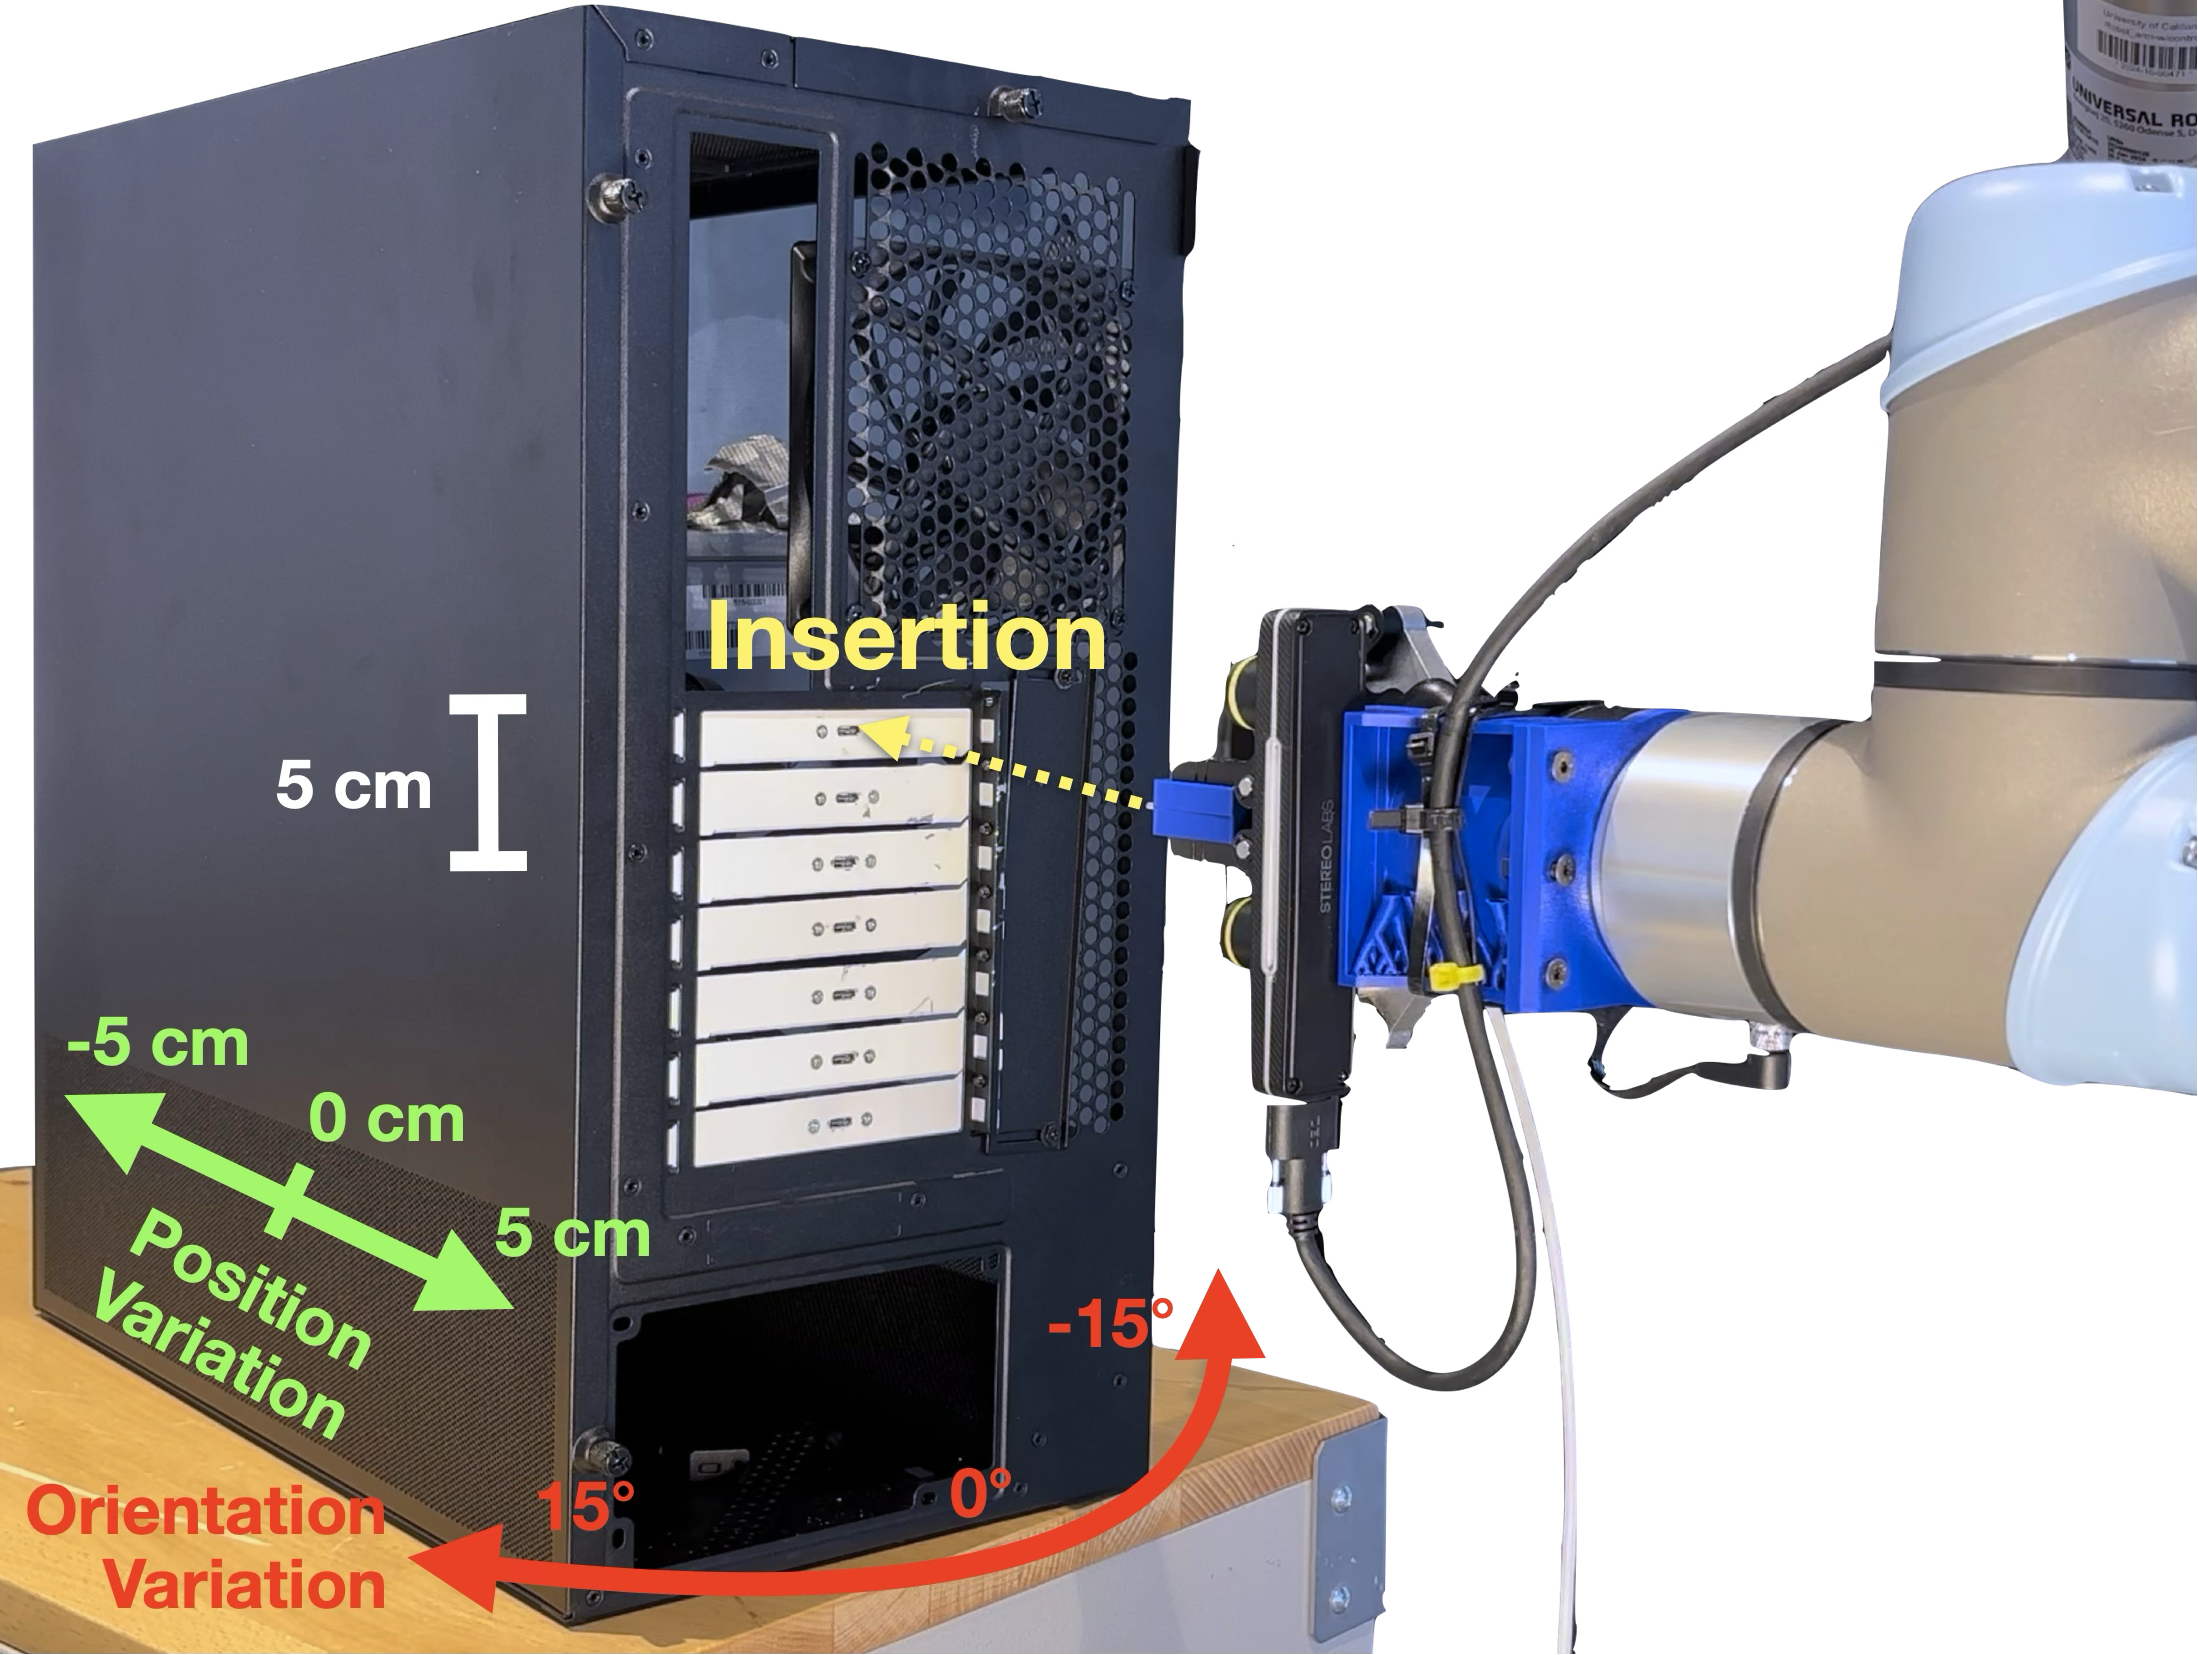
\includegraphics[width=0.9\linewidth]{figures/usb-insertion_setup.png}
        \captionof{figure}{Seven-ports cable insertion setup.}
        \label{fig:usb-insert-steup}
    \end{minipage}
    \hfill
     % The benchmark includes position, orientation, and insertion goal variations.
    % Right Side: The Table
    \begin{minipage}{0.48\textwidth}
        \centering
        \captionof{table}{\scriptsize \textbf{USB-C Cable insertion variations and results over 130 total insertion trials}. Success rates (SR) and execution time in seconds (ET). $^*$Excludes extraction phase.}
        \label{tab:benchmark-insertion}
        \scriptsize
\setlength{\tabcolsep}{4pt}
\renewcommand{\arraystretch}{0.95}
\begin{tabular}{lccc}
\toprule
\textbf{Variation} & \textbf{SR (Per trial)} & \textbf{SR (All)} & \textbf{ET (All)} \\
\midrule
\multicolumn{4}{c}{\textit{Insertion Goal Condition}} \\
\midrule
Individual port$^*$ & 5/5   & -   & 26.0 \\
Ascending order     & 32/35 & 2/5 & 247.0 \\
Descending order    & 32/35 & 4/5 & 223.2 \\
Odd index port      & 20/20 & 5/5 & 136.8 \\
Even index port     & 14/15 & 4/5 & 104.6 \\
\midrule
\multicolumn{4}{c}{\textit{Position/Orientation}} \\
\midrule
-$15^\circ$$^*$     & 4/5   & -   & 24.0 \\
$15^\circ$$^*$      & 5/5   & -   & 25.6 \\
-$5$ cm$^*$         & 5/5   & -   & 29.4 \\
$5$ cm$^*$          & 4/5   & -   & 28.0 \\
\bottomrule
\end{tabular}

    \end{minipage}
    
\end{figure}

For cable insertion benchmark evaluation, we utilize the computation graph generated by GaP, which operates via four modular ROS execution nodes: \textit{align to port}, \textit{touch port}, \textit{insert}, \textit{extract}. The robot first aligns to establish contact, generating a 1~$\times$1~$cm^2$ grid of insertion candidates. The \textit{insert} node then evaluates these positions, requiring $>$3~mm of progress at $<$10.0~N of force, and confirms successful insertion when the depth exceeds 6~mm at 30.0~N. Finally, the \textit{extract} node safely pulls the cable using a 2.0~Hz wiggling motion while maintaining lateral forces below 20.0~N. This entire policy requires approximately 30~seconds per insertion.

% Our policy works so that a robot pushes forward slowly until it establishes contact, creating a grid of insertion candidates within a 1~cm $\times$ 1~cm area near the contact plane. Then, the \textit{insert} node tests these candidate positions, verifying if the robot pushes forward by more than 3~mm while maintaining a force feedback below 10.0~N. A successful insertion is confirmed when the robot advances more than 6~mm as the force reaches 30.0~N. Finally, the \textit{extract} node applies a subtle 2.0~Hz wiggling motion to withdraw the cable, while keeping the lateral force under 20.0~N for safety. Our policy requires approximately 30 seconds per insertion. 


\begin{figure}
    \centering
    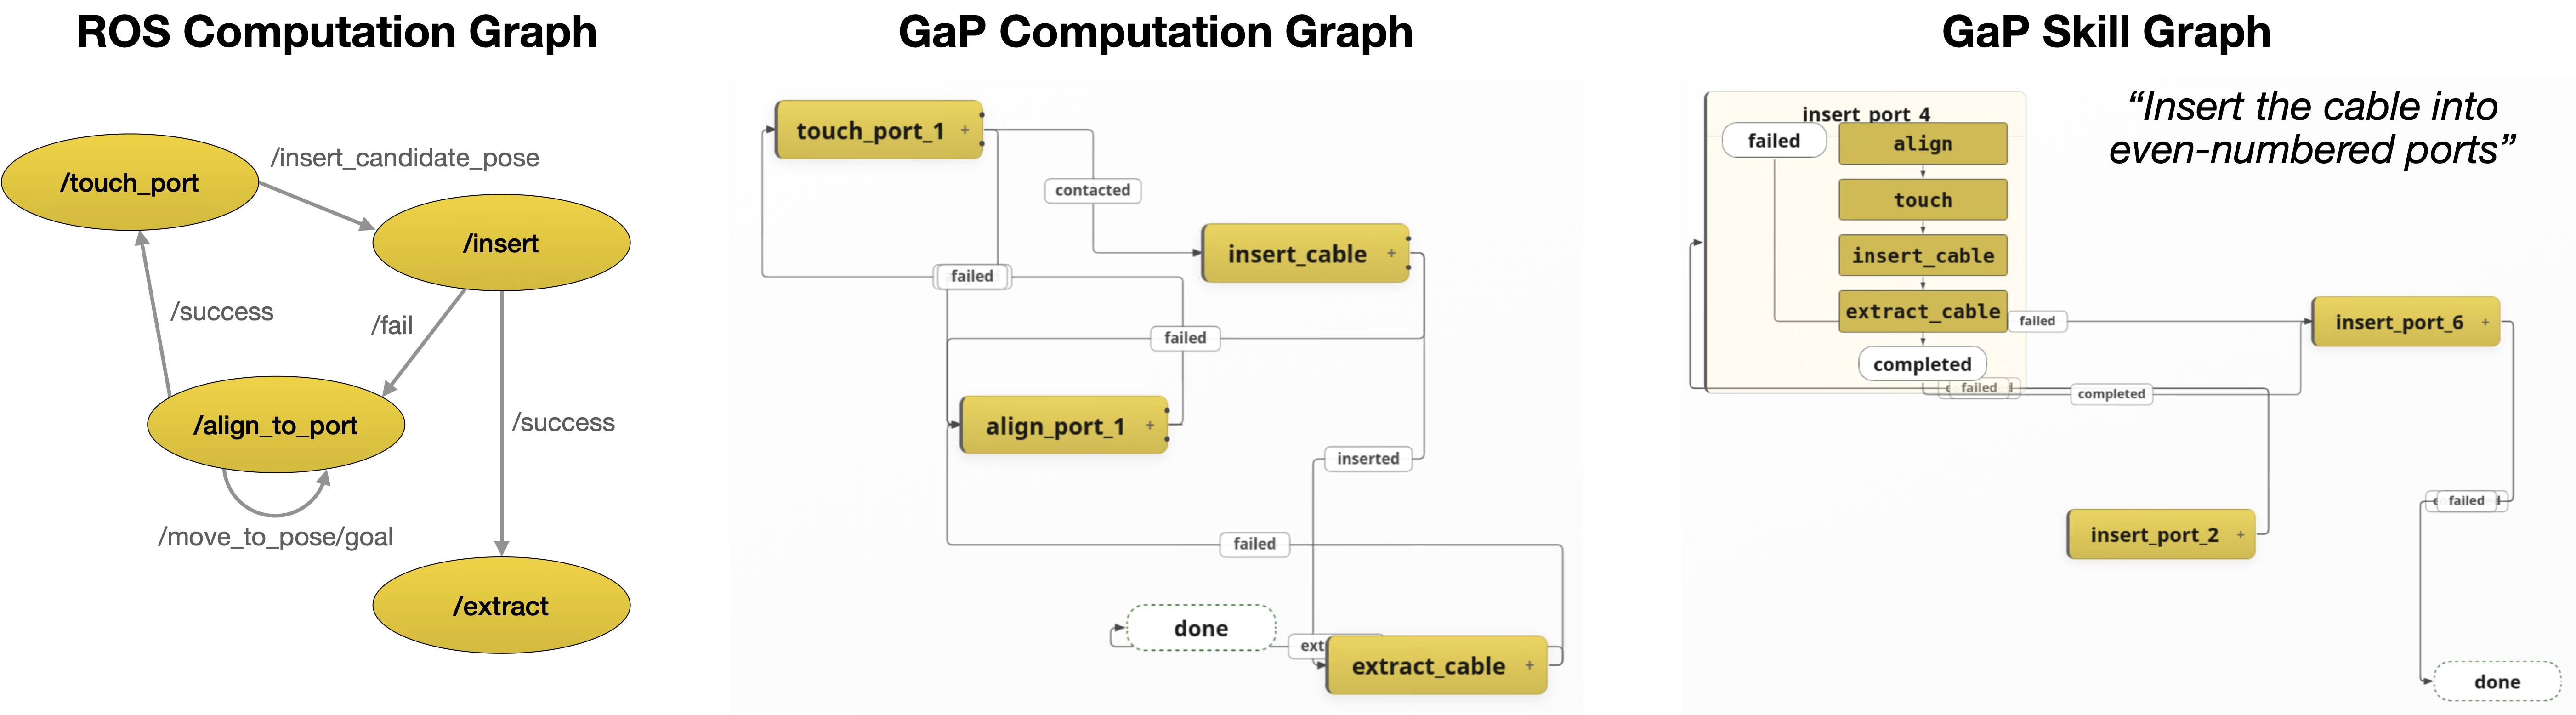
\includegraphics[width=1\linewidth]{figures/usb-insertion_graph.png}
    \caption{Left: ROS computation graph that is hand-engineered using traditional ROS nodes and topics. Middle: GaP can leverage nodes in ROS and generate a compatible graph using atomic skill sets, align to port, touch port, insert, and extract. Right: GaP can also use these nodes inside a subgraph for a long-horizon task, such as inserting the cable into even-numbered ports.}
    \label{fig:usb-insert-graph}
\end{figure}

\textbf{GaP provides flexibility to integrate with ROS nodes for robust, accurate task completion.} Across 130 insertion trials, GaP achieved a 0.93 success rate (121/130). A detailed breakdown is provided in Table~\ref{tab:benchmark-insertion}. GaP generated the correct workflows for all five text prompts, successfully handling long-horizon tasks with variations in position and orientation. Through this integration with ROS, GaP ensures both robust task execution and strong generalization across diverse positional variations and goal conditions. Some of the corresponding graphs generated by GaP are shown in Figure~\ref{fig:usb-insert-graph}.

% 

% \begin{figure}
%     \centering
%     \includegraphics[width=0.8\linewidth]{figures/cable_insertion.png}
%     \caption{\textbf{Physical Setup (Left), and GaP Graph Integration with ROS (Right) of Cable Insertion and Extraction with UR5e} \eric{placeholder figure, will replace with a complete figure showing UR5 and annotated with the sequence; Right hand side will be a figure showing how to connect GaP with ROS in this case (which ones are in ROS and which ones are in GaP)}}
%     \label{fig:cable}
% \end{figure}



\subsection{Benchmark V: Wash Crates (Simulation)}
\begin{wrapfigure}{r}{0.4\textwidth}
    \centering
    \vspace{-\baselineskip}
    \captionof{table}{\scriptsize \textbf{Wash Crates benchmark, 150 trials.} Success rate (SR), average cycle duration (s), and sustained throughput (successes/hr) over a 3-hour continuous run.}
    \label{tab:crate-wash}
    \scriptsize
    \resizebox{\linewidth}{!}{%
    \begin{tabular}{lccc}
    \toprule
    Method & SR & Avg(Dur) & Throughput\\
    \midrule
    Hand-Engineered & 0.99 & 176 & 19 \\
    GaP             & 0.95 & 179 & 18 \\
    \bottomrule
    \end{tabular}%
    }
    \vspace{6pt}
    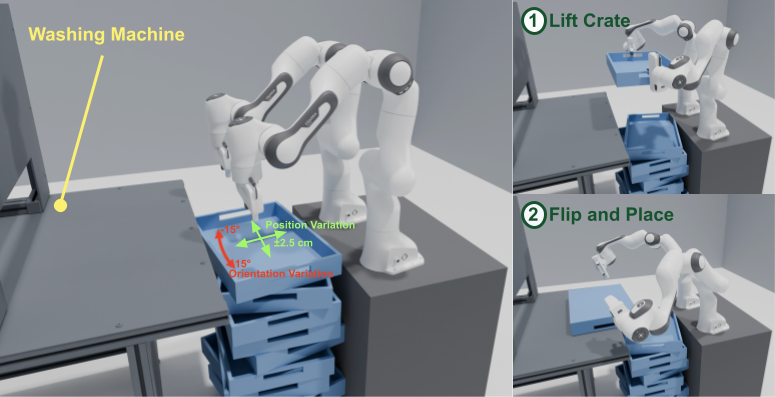
\includegraphics[width=0.95\linewidth]{figures/crate_washing.png}
    \caption{Industrial crate-washing setup.}
    \label{fig:crate-wash-setup}
    \vspace{-10pt}
\end{wrapfigure}
We compare GaP with a hand-engineered execution graph authored by an expert, representing the conventional manual engineering effort required in such settings. We run both policies over 150 trials sampled from the pose distribution, and additionally measure sustained throughput over a 3-hour continuous execution window.



\textbf{GaP closely matches an expert hand-engineered solution.} As reported in Table~\ref{tab:crate-wash}, GaP achieves a $0.953$ ($143/150$) success rate against the hand-engineered graph's $0.987$ ($148/150$), with similar average cycle times ($179.13$~s vs.\ $176.47$~s). Over the 3-hour throughput run both policies attempted $59$ trials, of which GaP completed $55$ and the hand-engineered graph $58$, corresponding to $18.33$ and $19.33$ successes per hour, respectively. These results suggest that GaP can autonomously produce coordinated bimanual policies whose reliability and throughput approach those of a manually hand-tuned baseline.